\documentclass[pt12]{article}
%.
\usepackage[margin=1in, paperwidth=8.5in, paperheight=11in]{geometry}
\usepackage{amsfonts}
\usepackage{amsmath}
\usepackage[margin=1in]{geometry}
\usepackage{amsfonts,amsmath,amssymb}
\usepackage[none]{hyphenat}
\usepackage{fancyhdr}
\usepackage{graphicx}
\usepackage{float}
\usepackage{xcolor}
\usepackage[nottoc,notlot,notlof]{tocbibind}
\usepackage{hyperref}
%.
\pagestyle{fancy}
\fancyhead{}
\fancyfoot{}
\fancyhead[L]{\slshape \MakeUppercase{Métodos de Monte Carlo - Quasi-Random}}
\fancyhead[R]{\slshape Erik Davino Vincent}
\fancyfoot[C]{\thepage}
%.
\makeatletter
\newcommand{\rmnum}[1]{\romannumeral #1}
\newcommand{\Rmnum}[1]{\expandafter\@slowromancap\romannumeral #1@}
\makeatother


\begin{document}

\begin{titlepage}

\title{\textbf{Relatório do Exercício Programa 3:\\Métodos de Monte Carlo - Quasi-Random}}
\author{Erik Davino Vincent - BMAC - Turma 54 \\ NUSP: 10736584}
\date{\today}
\maketitle
\line(1,0){440}
\ \\
\ \\
\ \\
\ \\
\ \\
\ \\
\ \\
\ \\
\begin{center}


\includegraphics[scale=0.1]{ime.png}\\
\ \\
\ \\
\begin{LARGE}\tt{IME - USP} \end{LARGE}


\end{center}

\end{titlepage}

\tableofcontents

\newpage

\begin{center}\section{Introdução}\end{center}
\

O seguinte texto tem por objetivo a análise de quatro métodos de Monte Carlo, utilizando geradores \textit{Quasi-Random}, visando a comparação entre a eficiência deles e a de geradores \textit{Pseudo-Aleatórios}, além do quanto são otimizados. Será discutido o tempo de computação de cada método, a comparação direta de seus resultados e a implementação para encontrar resultados bons, com erro $\leq1\% $.\\
\ 

Os métodos serão aplicados para calcular a estimativa da integral da função, no intervalo $ [0,1]$, definida por:
$$f(x) = e^{-\alpha x}\cos{\beta x} $$
onde $\alpha = 0.10736584$, o meu número USP e $\beta = 0.50886257$, o meu número de RG.\\

\subsection{Critério de Parada}
\ 
A escolha do critério de parada foi simples: se o programa estimar o erro que eu quero e este for $\leq 1\%$, o programa interrompe o processo e devolve os resultados. Exatamente o mesmo critério utilizado para o EP 2.\\ 
\ 

\section{Gerador escolhido}
\ 

A primeira decisão a ser tomada foi o gerador \textit{Quasi-Random} a ser utilizado. Encontrei uma boa biblioteca de geradores nos seguintes links: \href{http://people.sc.fsu.edu/~jburkardt/py_src/sobol/sobol.html}{Quasi-Random-Sobol}; \href{http://people.sc.fsu.edu/~jburkardt/py_src/halton/halton.html}{Quasi-Random-Halton}; \href{http://people.sc.fsu.edu/~jburkardt/py_src/van_der_corput/van_der_corput.html}{Quasi-Random-VanDerCorput}. (Cada um dos títulos anteriores é um link).\\
\ 

O gerador de sequencias de Sobol me pareceu interessante no primeiro momento, pois seu \textit{plotting} pode ser muito semelhante ao de um gerador \textit{pseudo-aleatório} uniforme normal, além de ser capaz de ter diferentes 'caras', definidas por uma \textit{seed}. Porém, o gerador que obtive era limitado a gerar sequencias de no máximo $n = 40$ valores. Logo, na implementação fiz com que para $n>40$ outra lista com $n-40$ valores fosse gerada, de forma recursiva, e concatenada à lista original (vide algorítimo). Dessa forma, também gerei um efeito de aleatoriedade, pois fiz com que a \textit{seed} fosse alterada para cada loop. Mas o problema que surgiu por essa implementação foi o tempo demasiadamente longo para a geração das listas, e consequentemente do calculo para resolver a integral e achar $n$ suficientemente grande para um erro $\epsilon < 1\%$.\\
\ 

Para o método \textit{Crud}, utilizando as sequencias de Sobol, obtive os seguintes resultados, para encontrar $\epsilon <1\%$:\\
\ 

\noindent Tempo de computação: $96$ segundos.\\
\noindent $\epsilon = 0.10499686985947774\%$ (lembrando que $\epsilon$ é a estimação do erro, assumindo distribuição normal).\\
\noindent Variância amostral = $0.16626400498125143$.\\
\noindent $n = 10000$ (lembrando que $n$ cresce a uma taxa de $10$ vezes).\\
\noindent $\hat{\gamma} = 0.7838860121075741$ (lembrando que $\hat{\gamma}$ é a estimação da integral de $f(x)$).\\
\ 

Como podemos ver o resultado é até mesmo pior do que vemos para uma distribuição \textit{pseudo-aleatória} uniforme, em termos de tempo de computação (para encontrar $\epsilon <1\%$):\\
\ 

\noindent Tempo de computação: $0.240$ segundos.\\
\noindent $\epsilon = 0.4822873755308176\%$ (lembrando que $\epsilon$ é a estimação do erro, assumindo distribuição normal).\\
\noindent Variância amostral = $0.16626400498125143$.\\
\noindent $n = 46656$ (lembrando que $n$ cresce a uma taxa de $2\sqrt{10}$ vezes).\\
\noindent $\hat{\gamma} = 0.7824057647774996$ (lembrando que $\hat{\gamma}$ é a estimação da integral de $f(x)$).\\
\ 

Por tal razão, fiz o mesmo teste para uma sequencia de \textit{VanDerCorput}, e os resultados foram tão bons, que utilizei a sequencia para o resto dos métodos. Vejamos os resultados (para encontrar $\epsilon <1\%$):\\
\ 

\noindent Tempo de computação: $0.371$ segundos.\\
\noindent $\epsilon = 0.4814989332265667\%$ (lembrando que $\epsilon$ é a estimação do erro, assumindo distribuição normal).\\
\noindent Variância amostral = $0.16313370287435794$.\\
\noindent $n = 46656$ (lembrando que $n$ cresce a uma taxa de $2\sqrt{10}$ vezes).\\
\noindent $\hat{\gamma} = 0.7824488038971255$ (lembrando que $\hat{\gamma}$ é a estimação da integral de $f(x)$).\\
\ 

Os resultados não são melhores do que da uniforme, para esse $n$, porém são muito semelhantes, e fixos para dados $n$, uma vez que a sequencia é sempre gerada da mesma maneira. Isso pode ser uma vantagem em relação ao gerador uniforme, uma vez que não possui aleatoriedade nos resultados. Para dado $n$, sempre terei valores garantidos.\\
\ 

\subsection{Gráficos das distribuições}
\ 

Antes de prosseguirmos, vejamos abaixo as distribuições/sequencias mencionadas acima, em uma área 1x1:\\
\ 

\textbf{UNIFORME:}\\
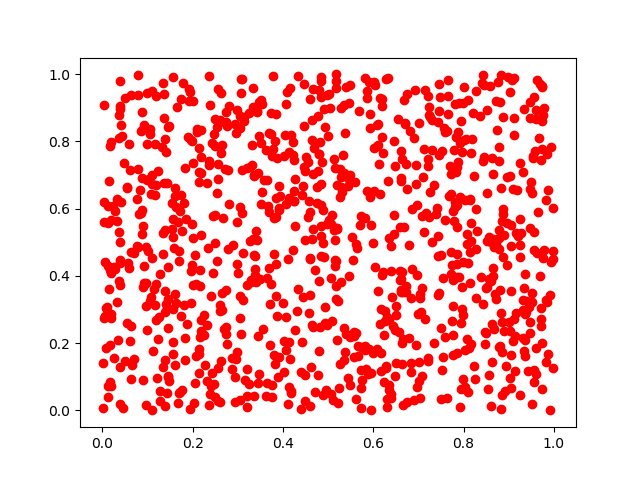
\includegraphics[scale=0.8]{uniform.png}\\
\newpage
\textbf{SOBOL:}\\
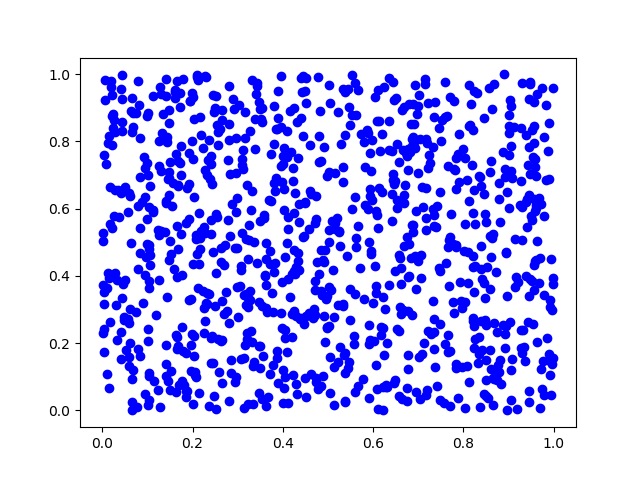
\includegraphics[scale=0.8]{sobol.png}\\
\ 

\textbf{VANDERCORPUT:}\\
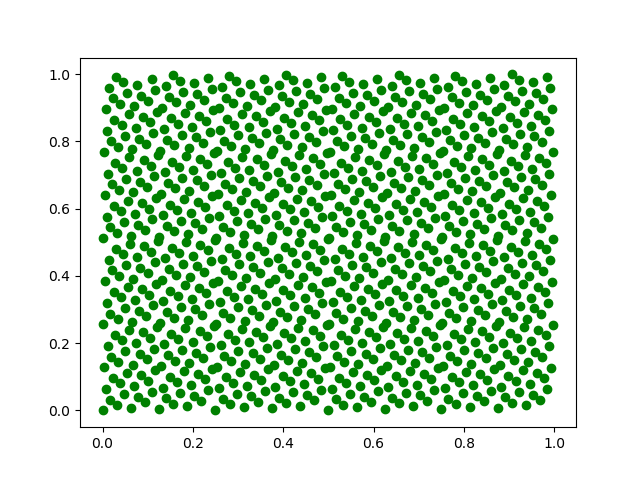
\includegraphics[scale=0.8]{van.png}\\
\ 

Como vemos, o gerador de Sobol e uniforme praticamente não apresentam diferenças notáveis. Além disso, vemos como o VanDerCorput possui distribuição muito bem comportada, o que, creio eu, permite um calculo muito mais preciso, especialmente para o caso do \textit{Hit-Or-Miss}. Verificaremos isso mais a frente.\\
\ 

\section{Método \textit{Crud}}
\ 

Em 2, praticamente cobrimos todo o básico para o método \textit{Crud}. Em termos de implementação, é idêntica a do EP 2, porém o gerador \textit{quasi-random} foi utilizado. Resta então fazer uma analise mais regrada, em termos de medidas, para qual gerador resulta em convergência mais rápida para $\hat{\gamma}$. Para isso, analisemos os gráficos:\\
\ 

Valor de $\hat{\gamma}$ até $n=1000$:\\
\indent \begin{small}laranja: \textit{quasi-random}; azul: uniforme.\end{small}\\
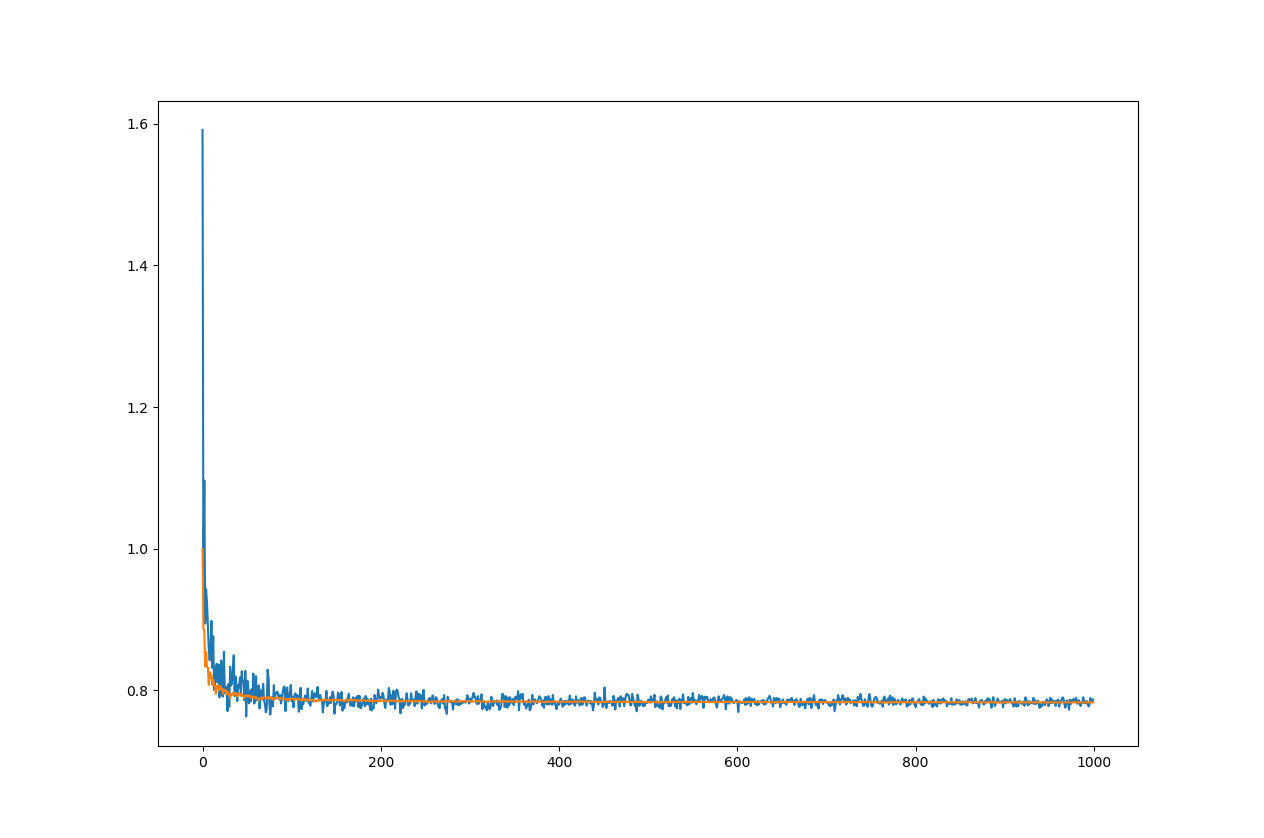
\includegraphics[scale=0.5]{conver_crud.png}\\
\ 

Como podemos ver, o gerador \textit{quasi-random} leva, por pouco, $\hat{\gamma}$ para o seu valor final mais rapidamente. Isso é, para um $n$ menor, o $\hat{gamma}$ \textit{quasi-random} está mais próximo do valor real da integral; ele converge mais rápido. Além disso ele é estável, diferente do aleatório uniforme, o que permite que mais vezes, o valor de $\hat{\gamma}$ esteja correto. De certa forma, a probabilidade do erro estar correto, por ser estimado, é maior. Isso significa que, pelo menos para esse método, o gerador \textit{quasi-aleatório} aumenta a eficiência. Não precisamos nos preocupar tanto com tempo de computação, uma vez que a convergência é mais rápida, e o tamanho de $n$ pode ser menor, para uma mesma precisão (ou até melhor).\\
\ 
\newpage

\section{Método \textit{Hit-or-Miss}}
\ 

A implementação utilizada foi a mesma que a do EP 2, porém, com o gerador aleatório trocado por um \textit{quasi-random} VanDerCorput. vejamos os resultados obtidos:\\
(Para encontrar erro $\epsilon<1\%$)\\
\ 

\textbf{Uniforme:}\\
\noindent Tempo de computação: $0.132$ segundos.\\
\noindent $\epsilon = 0.6818756060403957\%$ (lembrando que $\epsilon$ é a estimação do erro, assumindo distribuição normal).\\
\noindent Variância amostral = $0.002648060605982119$.\\
\noindent $n = 24300$. (lembrando que $n$ cresce a uma taxa de $2\sqrt{10}$ vezes).\\
\noindent $\hat{\gamma} = 0.7821399176954732$ (lembrando que $\hat{\gamma}$ é a estimação da integral de $f(x)$).\\
\ 

\textbf{\textit{VanDerCorput}:}\\
\noindent Tempo de computação: $0.209$ segundos.\\
\noindent $\epsilon = 0.6816896770211912\%$ (lembrando que $\epsilon$ é a estimação do erro, assumindo distribuição normal).\\
\noindent Variância amostral = $0.0026473385515386064$.\\
\noindent $n = 24300$. (lembrando que $n$ cresce a uma taxa de $2\sqrt{10}$ vezes).\\
\noindent $\hat{\gamma} = 0.7823045267489712$ (lembrando que $\hat{\gamma}$ é a estimação da integral de $f(x)$).\\
\ 

Vemos novamente resultados muito semelhantes entre as distribuições, com a opção \textit{quasi-random} apresentando erro e variância amostral menores do que a opção uniforme aleatória, com única desvantagem o tempo de computação levemente maior. Porém, para $n$ menor, vemos que a diferença de eficiência entre os métodos é ainda maior. Vejamos melhor com um gráfico:\\
\ 

Valor de $\hat{\gamma}$ até $n=1000$:\\
\indent \begin{small}laranja: \textit{quasi-random}; azul: uniforme.\end{small}\\
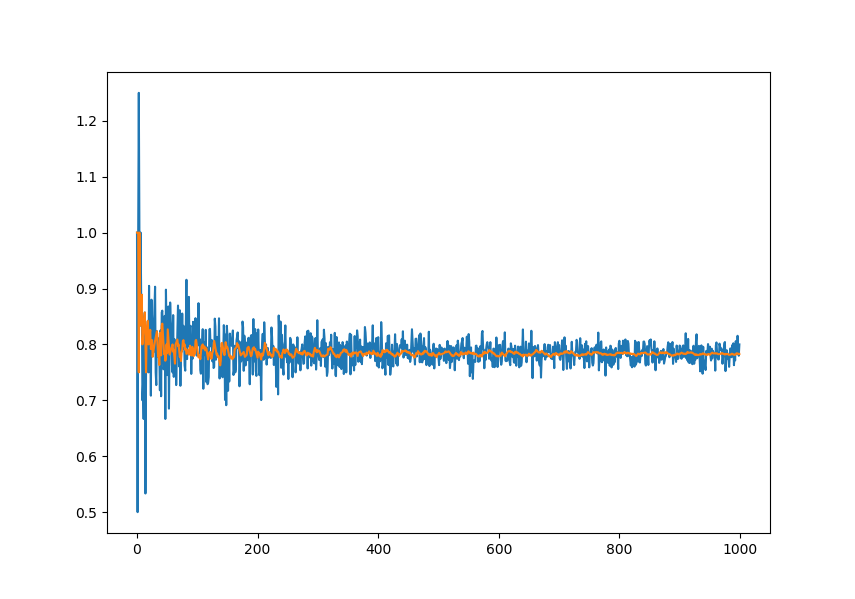
\includegraphics[scale=0.7]{conver_hit.png}
\newpage

A primeira coisa que podemos notar é que ambos os gráficos oscilam muito, e de forma decrescente. Isso é esperado do método, pois ele possui menos informações sobre $f(x)$. Diferente do gráfico na 3, vemos que a convergência se trata menos de qual 'chega' mais rápido (decai mais rapidamente) para o valor real da integral, mas sim de qual oscila menos, conforme chega mais próximo do valor real. Como podemos ver, a linha que representa o método pelo gerador \textit{quasi-random} oscila muito menos, o que nos permite, para cada $n$, ter mais certeza de que $\hat{\gamma}$ está fato mais próximos de $\gamma$. Vemos que essa diferença é ainda mais forte para $n$ menor. Vejamos um \textit{zoom} do gráfico acima, onde $n$ é pequeno:\\
\ 

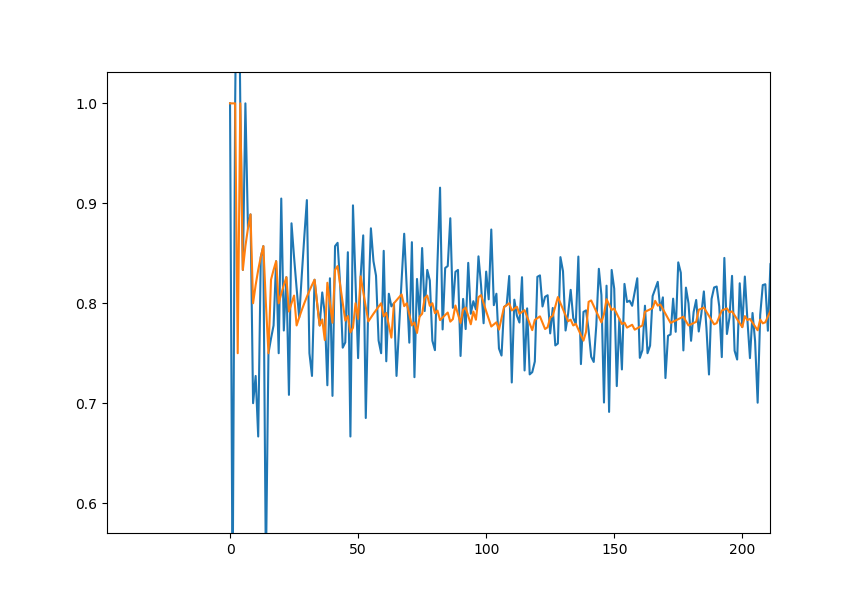
\includegraphics[scale=0.7]{conver_hit_zoom.png}\\
\ 

\section{\textit{Importance Sampling}}
\ 

Esse foi o método que mais sofreu modificações, porém não tao grandes. Primeiramente, não há geradores \textit{quasi-random} para todas as distribuições, logo, tive que criar a minha própria distribuição. De resto, a implementação é a mesma que a do EP 2.\\
\ 

O método em que me baseei para criação de geradores com distribuição de densidade de probabilidade aleatória para uma função $g(x)$ é feito da seguinte forma:

\begin{align}
\text{Seja $g(x)$ função integrável, tal que $G(x) = \int g(x)dx$, distribuição de densidade acumulada;}\\
\text{Se $G^{-1}(x)$ existe, e $x_{i}\sim U[0,1]$, então:}\\
u_{i} = G^{-1}(x_i) \Rightarrow u_{i}\sim g(x)
\end{align}
\newpage

Como não estamos utilizando uma distribuição uniforme, e a \textit{qusi-random VanDerCorput} simula bem uma uniforme, basta substituir $x_i \sim U[0,1]$ por $x_i \sim VanDerCorput$, obtendo uma distribuição \textit{quasi-random}, com 'cara' de $g(x)$.\\
\ 

\subsection{Escolha da $g(x)$}
\ 

Dessa vez, a escolha de $g(x)$ foi limitada a funções integráveis, e que as integrais fossem inversíveis. Não utilizei a distribuição beta, portanto. Ao invés disso, como a minha curva convenientemente se assemelha muito a uma reta, escolhi uma reta que passasse pelos pontos $(0,f(0))$ e $(1,f(1))$. A reta encontrada foi $g(x) = -0.40228x + 1$. Vejamos o gráfico:\\
\ 

\begin{center}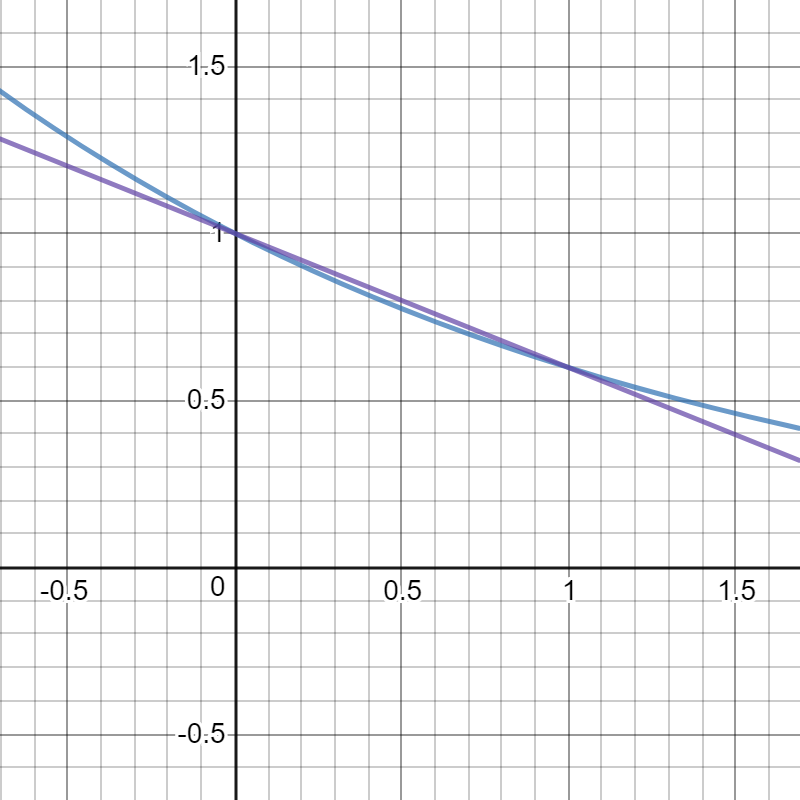
\includegraphics[scale=0.3]{desmos-graph.png}\end{center}
\ 

Porém, para essa reta ser uma distribuição de probabilidade em $[0,1]$, vale notar que $\displaystyle{G(x)\vert_{0}^{1} = 1}$. O resultado que obtive primeiramente foi $G(x) = x - 0.20114x^2$, onde $G(x)\vert_{0}^{1} = 0.79886$.
Para corrigir esse problema, somei ao valor obtido dessa integração o valor suficiente para resultar em $1$, que era $0.20114$, à $g(x)$. Logo, minha $g(x)$ final ficou $g(x) = -0.40228x+1.20114$, com $G(x) = 1.20114x - 0.20114x^2$. Vejamos o gráfico na página seguinte:\\
\ 

\begin{center}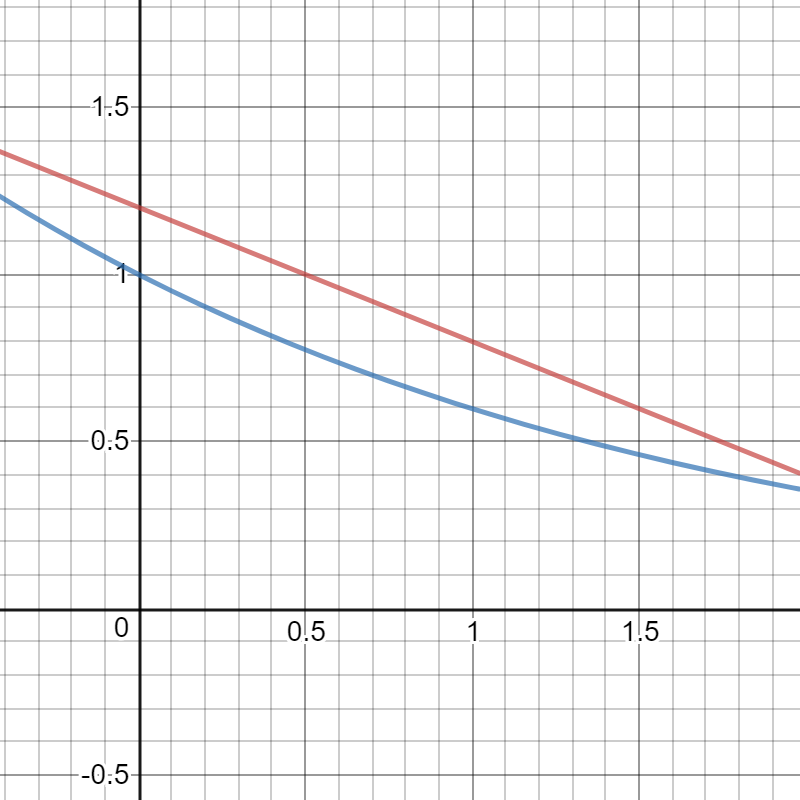
\includegraphics[scale=0.3]{desmos-graph(1).png}\end{center}
\ 

\subsubsection{Definição do gerador}
\

Com $g(x)$ e $G(x)$ definidas, bastava então criar o gerador \textit{quasi-random}. Para isso, primeiramente defini com a ajuda do \textit{Wolframalpha}, $G^{-1}(x)$:
$$G^{-1}(x) = 2.98583 \pm 0.0000497166\sqrt{3.60684\cdot 10^9 - 2.0114\cdot 10^9x}$$
A função criada (vide programa), consiste em transformar cada um dos $x_i$ elementos de uma sequencia de \textit{VanDerCorput} em $G^{-1}(x_i)$, e retornar uma nova lista \textit{quasi-random}.\\
\ 

\subsection{Resultados obtidos}
\ 

\textbf{Beta}\\
\noindent Tempo de computação: $2.51$ segundos.\\
\noindent $\epsilon = 0.4681088501408622\%$ (lembrando que $\epsilon$ é a estimação do erro, assumindo distribuição normal).\\
\noindent Variância amostral = $0.044354512807987204$.\\
\noindent $n = 7776$. (lembrando que $n$ cresce a uma taxa de $2\sqrt{10}$ vezes).\\
\noindent $\hat{\gamma} = 0.7853107345425413$ (lembrando que $\hat{\gamma}$ é a estimação da integral de $f(x)$).\\
\ 

\textbf{\textit{VanDerCorput - g(x)}:}\\
\noindent Tempo de computação: $0.00097$ segundos.\\
\noindent $\epsilon = 0.59559405970736\%$ (lembrando que $\epsilon$ é a estimação do erro, assumindo distribuição normal).\\
\noindent Variância amostral = $0.000664846013250364$.\\
\noindent $n = 72$. (lembrando que $n$ cresce a uma taxa de $2\sqrt{10}$ vezes).\\
\noindent $\hat{\gamma} = 0.783542216119383$ (lembrando que $\hat{\gamma}$ é a estimação da integral de $f(x)$).\\
\ 

Esse resultado me espantou. Não há sombra de duvidas para a maior do eficiência do \textit{quasi-random} para este método, basta ver os resultados (a comparação ideal seria utilizar o gerador de distribuição $g(x)$ aleatório para encontrar os resultados do \textit{importance sampling} aleatório). Não apenas em relação ao gerador Beta e o método aleatório, mas também em relação a todos os outros métodos apresentados. Vejamos os gráficos de convergência para reforçar a conclusão sobre esse resultado:\\


Valor de $\hat{\gamma}$ até $n=1000$:\\
\indent \begin{small}laranja: \textit{quasi-random}; azul: uniforme.\end{small}\\
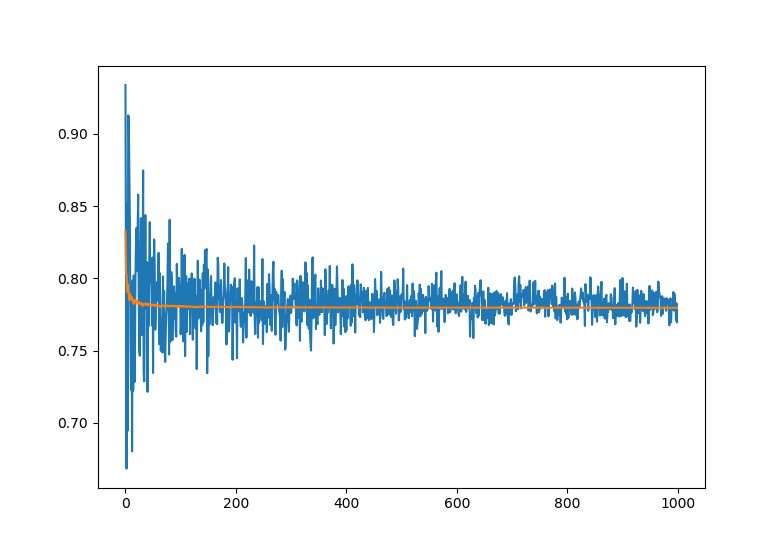
\includegraphics[scale=0.7]{conver_smp.png}
\ 

\section{\textit{Control Variance}}
\ 

O ultimo método, como os demais, também seguiu a mesma implementação do EP 2, apenas com o gerador uniforme, trocado pelo \textit{quasi-random}. Vejamos os resultados obtidos:\\
\ 

\textbf{Uniforme}\\
\noindent Tempo de computação: $2.257$ segundos.\\
\noindent $\epsilon = 0.473428652971247\%$ (lembrando que $\epsilon$ é a estimação do erro, assumindo distribuição normal).\\
\noindent Variância amostral = $0.04536837112649993$.\\
\noindent $n = 7776$. (lembrando que $n$ cresce a uma taxa de $2\sqrt{10}$ vezes).\\
\noindent $\hat{\gamma} = 0.7852965541990419$ (lembrando que $\hat{\gamma}$ é a estimação da integral de $f(x)$).\\
\ 

\textbf{\textit{VanDerCorput - g(x)}:}\\
\noindent Tempo de computação: $0.005983114242553711$ segundos.\\
\noindent $\epsilon = 1.2057739535976042\cdot 10^{-05}\%$ (lembrando que $\epsilon$ é a estimação do erro, assumindo distribuição normal).\\
\noindent Variância amostral = $4.385380947269368\cdot 10^{-15}$.\\
\noindent $n = 2$. (lembrando que $n$ cresce a uma taxa de $2\sqrt{10}$ vezes).\\
\noindent $\hat{\gamma} = 0.7824294083396494$ (lembrando que $\hat{\gamma}$ é a estimação da integral de $f(x)$).\\
\ 

Vejamos primeiramente o gráfico:\\
\newpage

Valor de $\hat{\gamma}$ até $n=1000$:\\
\indent \begin{small}laranja: \textit{quasi-random}; azul: uniforme.\end{small}\\
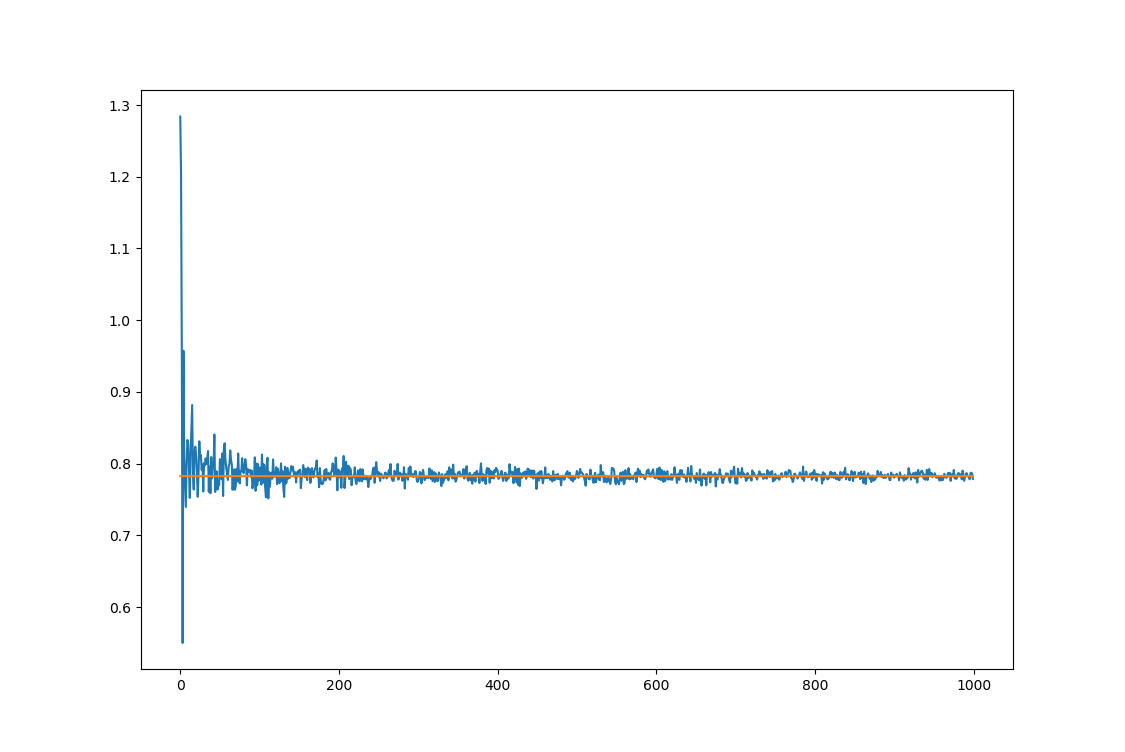
\includegraphics[scale=0.6]{conver_var.png}
\ 

O resultado pode parecer surpreendente, porém, pela forma como funciona esse método, o que acontece é que não importa o $n$, se usarmos o \textit{quasi-random}. Na verdade o fator que afeta o resultado dessa estimativa é somente a precisão de $\displaystyle{\int_{0}^{1} \phi(x)}$ (lembrando que $\phi(x)$ é a função de controle que se assemelha a $f(x)$). Minha suposição é de que $\phi(x)$ se assemelha tanto a $f(x)$ que a variância e covariância de $f(x)$ e $\phi(x)$ aproximam $\hat{\gamma}$ de $\int\phi(x) dx$ para um $n$ muito pequeno, isso é: 1. Assim, todo o cálculo depende então da precisão de $\int\phi(x)dx$.\\
\ 

Isso me leva a supor que, caso não seja possível encontrar uma função alternativa $\phi(x)$ tão próxima de $f(x)$, esse resultado não seria tão bom.\\
\ 

\section{Consideração final}
\ 

Pelos resultados obtidos, é seguro afirmar que, ao menos para a função em questão os geradores \textit{quasi-random} produzem resultados com precisão muito melhor, de forma geral. É difícil tirar conclusões do que aconteceria caso usássemos outras funções. Mas minha melhor suposição é de que, o método \textit{Hit-or-Miss} e o \textit{Importance Sampling} seriam os que produziriam sempre os melhores resultados, se comparado ao uso dos geradores aleatórios convencionais.









\end{document}
